\documentclass[12pt, a4paper]{article}
\usepackage[T2A]{fontenc}
\usepackage[utf8]{inputenc}
\usepackage[russian]{babel}
\usepackage{graphicx}
\usepackage{geometry}
\usepackage{textpos}
\usepackage{textpos}
\usepackage{array}
\usepackage{caption}
\usepackage{amsmath}
\usepackage{fancyhdr}

\geometry{
	a4paper,
	textwidth=170mm,
	textheight=250mm,
	left=20mm,
	top=20mm,
}

\newcommand{\Faculty}{Робототехника и комплексная автоматизация}
\newcommand{\Department}{Системы автоматизированного проектирования (САПР)}

\newcommand{\TitleText}{Расчетно-пояснительная записка}
\newcommand{\Title}{{\Huge \textbf{\TitleText}}}

\newcommand{\SubTitleText}{к курсовой работе по дисциплине \\ "Разработка информационных систем"}
\newcommand{\SubTitle}{{\Huge \textbf{\SubTitleText}}}

\newcommand{\FullName}{Дунайцев Александр Иванович}
\newcommand{\Author}{Дунайцев А. И}
\newcommand{\EduGroup}{РК6-54Б}
\newcommand{\TaskType}{Расчетно поятснительная записка}
\newcommand{\WorkTheme}{Разработка информационной системы "История болезни"}

% Пример как добавить картину в документ
%\begin{figure}[h]
%	\centering    % Центрируем
%	\includegraphics[width=0.25\textwidth]{pic.png}
%	\caption{a nice plot} % Подписть к картинке, будет снизу
%	\label{fig:pic1} % Можно указывать ссылку на эту картинку в тексте, как \ref{fig:pic1}
%\end{figure}


%\title{Заголовок документа}
%\author{Студент кафедры РК6 МГТУ им. Н. Э. Баумана Дунайцев А. И.}
%\date{October 2021}

\setlength{\columnsep}{1in}


\begin{document}
	% Место для верстки титульного документа
	\thispagestyle{empty}
	\begin{tabular}{m{0.15\linewidth}m{0.85\linewidth}}
		\centering
		
\includegraphics[scale=0.07]{static/bmstu.pdf} &
		{\centering
			Министерство науки и высшего образования Российской Федерации
			Федеральное государственное бюджетное образовательное учреждение
			высшего образования
			
			«Московский государственный технический университет
			имени Н.Э. Баумана
			(национальный исследовательский университет)»
			
			(МГТУ им. Н.Э. Баумана)
			
		} \\
		\hline
		\multicolumn{1}{p{0.15\textwidth}}{} & \multicolumn{1}{p{0.85\textwidth}}{} \\
		\multicolumn{1}{p{0.15\textwidth}}{ФАКУЛЬТЕТ}	&	\multicolumn{1}{p{0.85\textwidth}}{\Faculty}	\\
		\multicolumn{1}{p{0.15\textwidth}}{КАФЕДРА}	&	\multicolumn{1}{p{0.85\textwidth}}{\Department}	\\
	\end{tabular}
	\vfil
	
	{\centering
		\Title
		
		\SubTitle
	}
	
	\vfil
	\begin{center}
		\begin{tabular}{p{0.3\textwidth}p{0.4\textwidth}} 
			Студент:	& \FullName \\ 
			\hline
			Группа:	& \EduGroup \\ 
			\hline
			%Тип задания:	& \TaskType \\ 
			%\hline
			Тема:	& \WorkTheme \\ 
			\hline
		\end{tabular}
	\end{center}
	
	\vfil
	
	\begin{tabular}{p{0.45\textwidth}p{0.25\textwidth}p{0.25\textwidth}} 
		\large
		Студент	&	$\underset{\text{подпись, дата}}{\underline{\hspace{0.2\textwidth}}}$ & \underline{\Author}  \\ 
		& & \\
		Преподаватель	&	$\underset{\text{подпись, дата}}{\underline{\hspace{0.2\textwidth}}}$ & \underline{Увайсова А. С.} \\ 
	\end{tabular}
	
	\vfil
	\vfil
	\begin{center}
		Москва, 2021
	\end{center}
	
	%Конец титульного листа
	\newpage	
	% Страница с версткой содержания
	\tableofcontents
	\newpage
	
	% Далее идут секции с текстом документа
	\section{Аннотация.}
	Курсовой проект включает в себя реализацию параметризованных запросов через пользовательский интерфейс, авторизацию пользователей, проект и реализацию основного бизнес-процесса, а также работу с хранимыми процедурами.
	
	Была составлена UML диаграмма ролей конечных пользователей. Для каждой роли
	предусмотрены соответствующие варианты использования информационной системы.
	
	Для разработки информационной системы, в рамках данного курсового проекта, были использованы следующие программыне средства, языки программирования и технологии: язык программирования общего назначения python, фреймворк для создания веб-приложений на языке python Flask, язык гиперразметки HTML, декларативный язык программирования запросов к реялционным базам данных SQL, система управления базами данных MySQL, набор инструментов для создания сайто Bootstrap.
	
	\section{Задание. Описание предметной области.}
	В рамках курсового проекта необходимо разработать информационную систему, состоящую
	из базы данных и интерфейса конечного пользователя. В интерфейсе конечного
	пользователя должно быть предусмотрено 4 варианта использования: Главное меню, работа
	с запросами, авторизация и основной бизнес-процесс. Для каждого варианта использования
	необходимо сделать:
	
	\begin{itemize}
		\item Сценарий
		\item BPMN-диаграмму контроллера
		\item Требования к шаблонам
		\item Программная архитектруа реализации вариантовиспольования
	\end{itemize}
	
	\section{Определение конечных пользователей.}
	В разрабатываемой информационной системе определим 3 вида конечных пользователей:
	\begin{itemize}
		\item Администратор
		\item Главный врач
		\item Врач
	\end{itemize}
    \newpage

    \section{Разработка UML диаграммы вариантов использования.}
	\begin{figure}[ht!]
		\centering    % Центрируем
		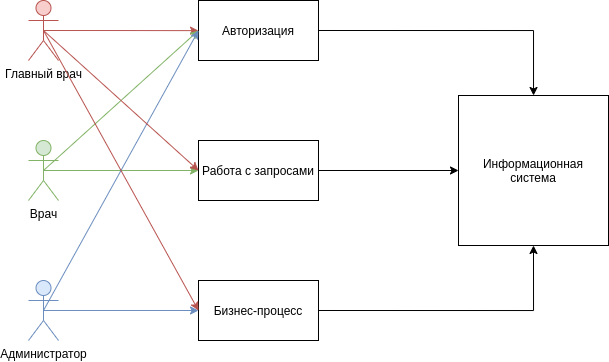
\includegraphics[width=0.7\textwidth]{pictures/UML_variants_using.png}
		\caption{UML диаграмма вариантов использования.} % Подписть к картинке, будет снизу
		\label{fig:pic1} % Можно указывать ссылку на эту картинку в тексте, как \ref{fig:pic1}
	\end{figure}

   \section{Вариант использования "Главное меню".}
   
   Количество пунктов в главном меню соответствует количеству вариантов использования
   плюс пункт для выхода из системы.
   
   При запуске ИС управление передается контроллеру главного меню.
   
   \subsection{Сценарий работы главного меню.}
   \begin{itemize}
   	\item Пользователь запускает сценарий.
   	\item Система присылает главное меню.
   	\item Пользователь выбирает один из пунктов (вариантов использования).
   	\item Система передаёт управление контроллеру соответствующего варианта
   	использования.
   \end{itemize}
   \newpage

   \subsection{BPMN диаграмма контроллера главного меню.}
   \begin{figure}[ht!]
   	\centering    % Центрируем
   	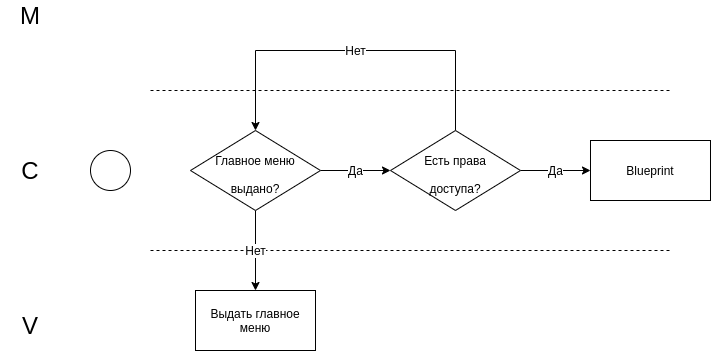
\includegraphics[width=0.8\textwidth]{pictures/BPMN_main_menu_using.png}
   	\label{fig:pic2} % Можно указывать ссылку на эту картинку в тексте, как \ref{fig:pic1}
   	\caption{BPMN диаграмма контроллера главного меню.}
   \end{figure}

   \subsection{Требования к шаблонам.}
   
   Статический шаблон Главное меню.
   \\
   Меню содержит следующие ссылки:
   \begin{itemize}
   	\item На контроллер работы с запросами (адрес '/db\_requests')
   	\item На выход из системы (адрес '/exit')
   \end{itemize}

	\newpage
	\subsection{Программная архитектура реализации главного меню.}
	 \begin{figure}[ht!]
		\centering    % Центрируем
		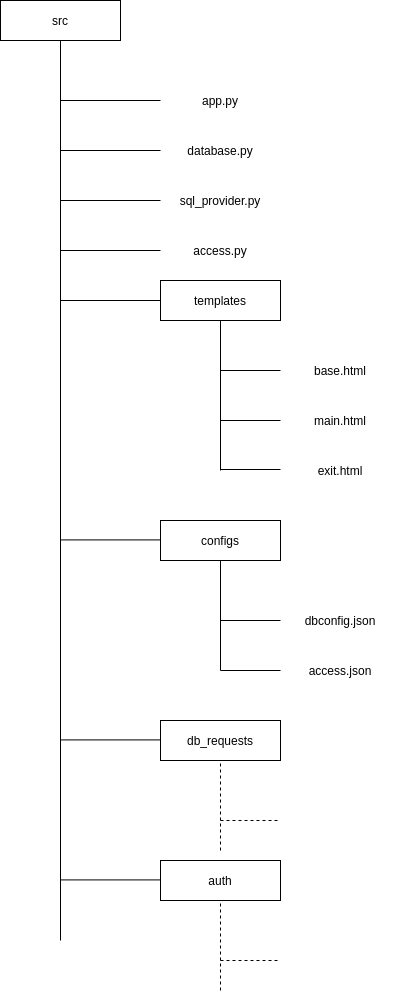
\includegraphics[height=0.7\textheight]{pictures/main_menu_arch.png}
		\label{fig:pic3} % Можно указывать ссылку на эту картинку в тексте, как \ref{fig:pic1}
		\caption{Программная архитектура реализации главного меню.}
	\end{figure}

   \section{Вариант использования «Работа с запросами».}
   \subsection{Сценарий использования "Работа с запросами".}
   \begin{itemize}
   	\item Пользователь запускает сценарий.
   	\item Система присылает меню запросов.
   	\item Пользователь выбирает запрос.
   	\item Система присылает форму для ввода параметров.
   	\item Пользователь вводит параметры.
   	\item Система выполняет запрос и присылает пользователю страницу с результатами
   	запроса и ссылкой для возврата в меню запросов.
   \end{itemize}
   
   \subsection{BPMN диаграмма контроллера меню запросов.}
   \begin{figure}[ht!]
   	\centering    % Центрируем
   	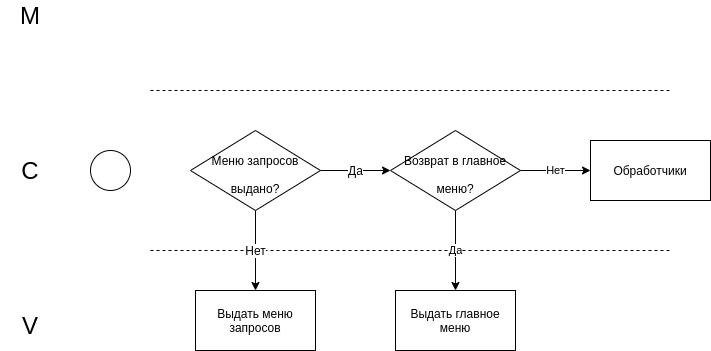
\includegraphics[width=0.8\textwidth]{pictures/Requests_Controller.png}
   	\label{fig:pic4} % Можно указывать ссылку на эту картинку в тексте, как \ref{fig:pic1}
   	\caption{BPMN диаграмма контроллера меню запросов.}
   \end{figure}

    \begin{figure}[ht!]
    	\centering    % Центрируем
    	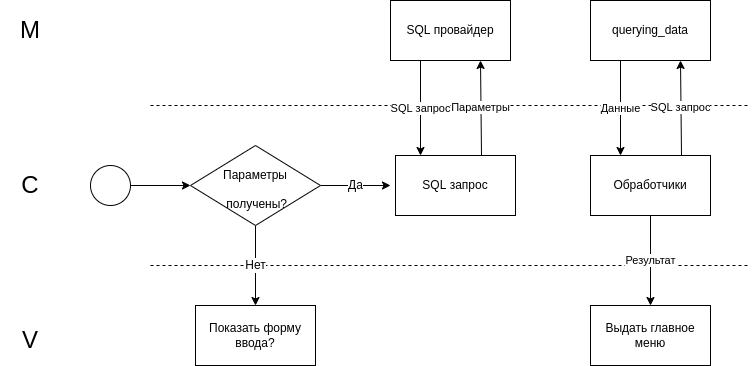
\includegraphics[width=0.8\textwidth]{pictures/requestHandlerBPMN.png}
    	\label{fig:pic5} % Можно указывать ссылку на эту картинку в тексте, как \ref{fig:pic1}
    	\caption{BPMN диаграмма обработчика конкретного запроса.}
    \end{figure}
    
    \subsection{Требования к шаблонам.}
    Меню запросов сожержит следующие ссылки:
    \begin{itemize}
    	\item На страницу для выполнения запроса 1 (адрес '/rquests/1')
    	\item На страницу для выполнения запроса 2 (адрес '/rquests/2')
    	\item На страницу для выполнения запроса 3 (адрес '/rquests/3')
    	\item На страницу для выполнения запроса 4 (адрес '/rquests/4')
    	\item На возврат в главное меню (адрес /)
    \end{itemize}

    Страница каждого из запросов содержит форму для ввода параметров запроса и ссылку
    (адрес ‘/requests’) на возврат в меню запросов. Форма в свою очередь должна иметь кнопку
    для отправки введённых параметров и перехода по ссылке ‘/requests/result’.
    
    Страница, отображающая результаты запроса, должна представлять их в виде таблицы. Под
    таблицей должна находиться ссылка (адрес ‘/reqeusts’) для возврата в меню запросов.
    
    \subsection{Программная архитектура реализации работы с запросами.}
    \begin{figure}[ht!]
    	\centering    % Центрируем
    	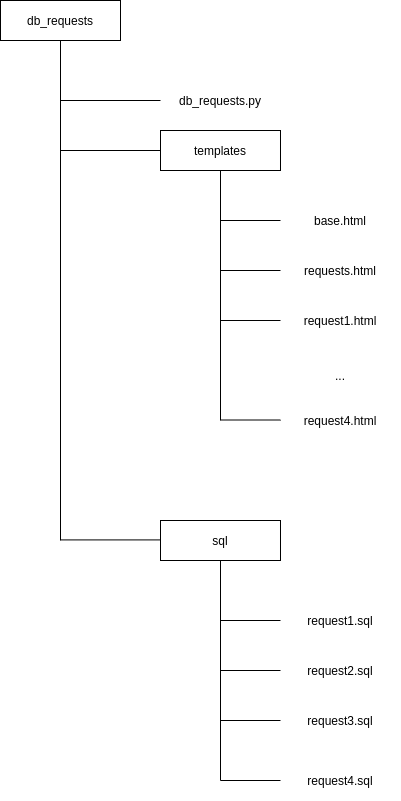
\includegraphics[height=0.6\textheight]{pictures/requests_arch.png}
    	\label{fig:pic6} % Можно указывать ссылку на эту картинку в тексте, как \ref{fig:pic1}
    	\caption{Программная архитектура реализации работы с запросами.}
    \end{figure}
    \newpage
    
    \section{Вариант использования «Авторизация». }
	\subsection{Сценарий работы «Авторизация».}
	\begin{itemize}
		\item Пользователь запускает сценарий.
		\item Система возвращает форму ввода логина и пароля.
		\item Пользователь вводит данные и нажимает кнопку отправить.
		\item {Система проверяет введённые данные и возвращает сообщение об успешной
		       авторизации, если такие логин и пароль существуют в БД, и сообщение об ошибке,
	      	   если пользователя с таким логином и паролем в БД нет.}
	\end{itemize}

    \subsection{BPMN диаграмма контроллера авторизации.}
    \begin{figure}[h]
    	\centering    % Центрируем
    	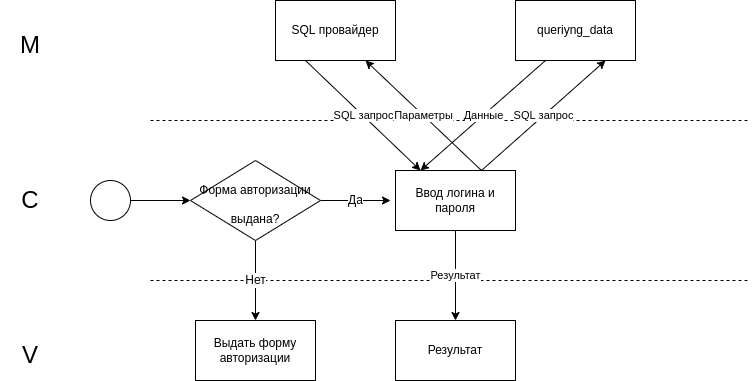
\includegraphics[width=0.8\textwidth]{pictures/authBPMN.png}
    	\label{fig:pic7} % Можно указывать ссылку на эту картинку в тексте, как \ref{fig:pic1}
    	\caption{BPMN диаграмма контроллера авторизации.}
    \end{figure}

    \subsection{Требования к шаблонам.}
    Страница авторизации сдержит форму для ввода логина и пароля, кнопку для отправки
    обработчику введённых данных, кнопку для очистки сессии (переход по адресу ‘/login/clearsession’) и ссылку на возврат в главное меню (адрес ‘/’).
    
    При вводе верного логина и пароля после нажатия кнопки отправки должна отобразиться
    страница с подтверждение, содержащая ссылку для перехода в главное меню.
    
    При вводе неверного логина или пароля после нажатия кнопки отправки должна
    отобразиться страница с сообщением об ошибке, содержащая ссылку для перехода в меню
    запросов (адрес ‘/login’), для повторного ввода данных, и ссылка для перехода в главное
    меню.
    
    При нажатии кнопки для очистки сессии должна отобразиться страница с сообщением об
    успешной очистке сессии и ссылкой для перехода в главное меню.
    
    \newpage
    \subsection{Программная архитектура реализации авторизации.}
    \begin{figure}[ht!]
    	\centering    % Центрируем
    	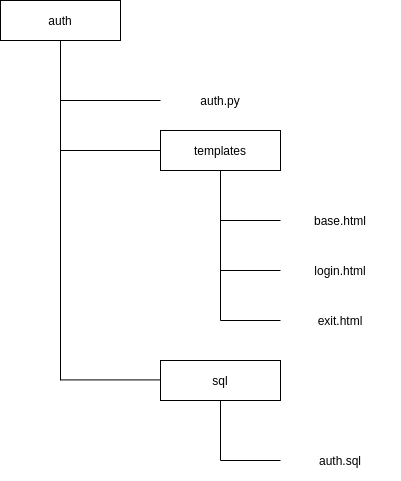
\includegraphics[height=0.4\textheight]{pictures/auth_arch.png}
    	\label{fig:pic8} % Можно указывать ссылку на эту картинку в тексте, как \ref{fig:pic1}
    	\caption{BPMN диаграмма контроллера авторизации.}
    \end{figure}

    \section{Вариант использования "Запись пациентов на госпитализацию".}
    \subsection{Сценарий использования "Запись пациентов на госпитализацию".}
    
    \begin{itemize}
    	\item {Пользователь запускает сценарий.}
    	\item {Система присылает форму записи пациентов, имеющих направление на госпитализацию.}
    	\item {Пользователь выбирает пациента и проверяет его паспортные данные.}
    	\item {Система выдает список врачей и доступных палат, в которых можно разместить пациента.}
    	\item {Пользователь выбирает для пациента врача и палату из доступных.}
    	\item {Система выполняет запрос и вносит изменения в базу данных. Создается новая запись о пациенте и его истории болезни в соответствующих таблицах.}
    \end{itemize}

    В случае, если мест в палатах нет, пациент сможет быть госпитализирован только после того, как места в палатах освободятся.
	
	\subsection{BPMN диаграмма контроллера записи пациентов.}
	\begin{figure}[ht!]
		\centering    % Центрируем
		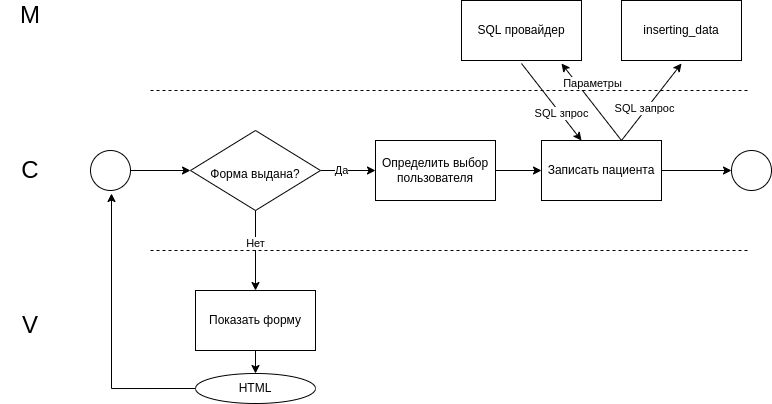
\includegraphics[width=0.8\textwidth]{pictures/referralGospitalize.png}
		\label{fig:pic9} % Можно указывать ссылку на эту картинку в тексте, как \ref{fig:pic1}
		\caption{BPMN диаграмма контроллера записи пациентов на госпитализацию.}
	\end{figure}

   \subsection{Требования к шаблонам.}
   
   Страница с сценарием "Запись пациента на госпитализацию" содержит три поля, обязательных для выбора. Первое поле содержит список фамилий и паспортных данных паицентов, имеющих направление на госпитализацю. Второе поле позволяет сделать выбор палаты, в которой есть место, чтобы разместить пациента. Также для каждой палаты отображено, какое количество людей в ней уже есть. Третье поле позволяет выбрать врача для пациента. Также, чтобы передать выбранные параметры в систему, на странице предусмотрена соответствующая кнопка.
   
   При отсутствии свободных мест в платах, пользователь не может записать пациента на госпитализацию до тех пор, пока место в одной из палат не освободится.
   
   \newpage
   \subsection{Программная аритектура реализации сценария "Запись пациента на госпитализацю".}
   \begin{figure}[ht!]
   	\centering    % Центрируем
   	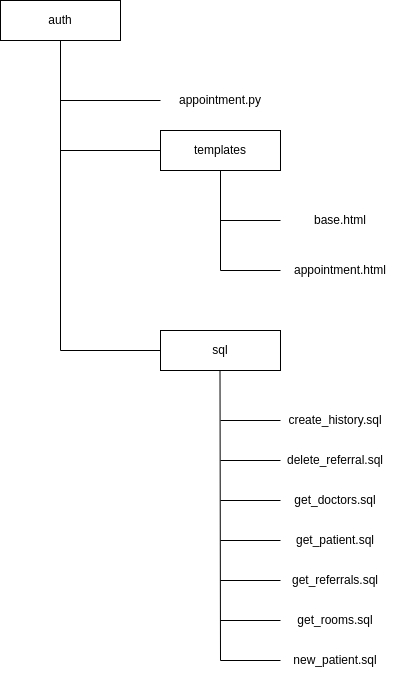
\includegraphics[height=0.5\textheight]{pictures/archReferral.png}
   	\label{fig:pic10} % Можно указывать ссылку на эту картинку в тексте, как \ref{fig:pic1}
   	\caption{Программная аритектура реализации сценария "Запись пациента на госпитализацю".}
   \end{figure}

   \section{Вариант использования "Лечение пациента".}
   \subsection{Сценарий использования "Лечение пациента".}
   
   \begin{itemize}
   	\item {Пользователь запускает сценарий.}
   	\item {Открывает форму выбора пациента.}
   	\item {Пользователь выбирает пациента для проведения осмотра.}
   	\item {Система получает информацию о выбраном пациенте и отображает страницу с историей болезни пациента.}
   	\item {Пользователь вносит записи в исорию болезни.}
   	\item {Система отображает внесенные записи в соответствующем поле на странцие истории болезни.}
   	\item {Пользователь выписывает пациента.}
   	\item {Система вносит изменения в историю болезни и закрывает ее. Затем система возвращает пользователя к странице выбора пациентов.}
   \end{itemize}

    \subsection{BPMN диаграмма контроллера "Лечение пациента".}
    \begin{figure}[h]
    	\centering    % Центрируем
    	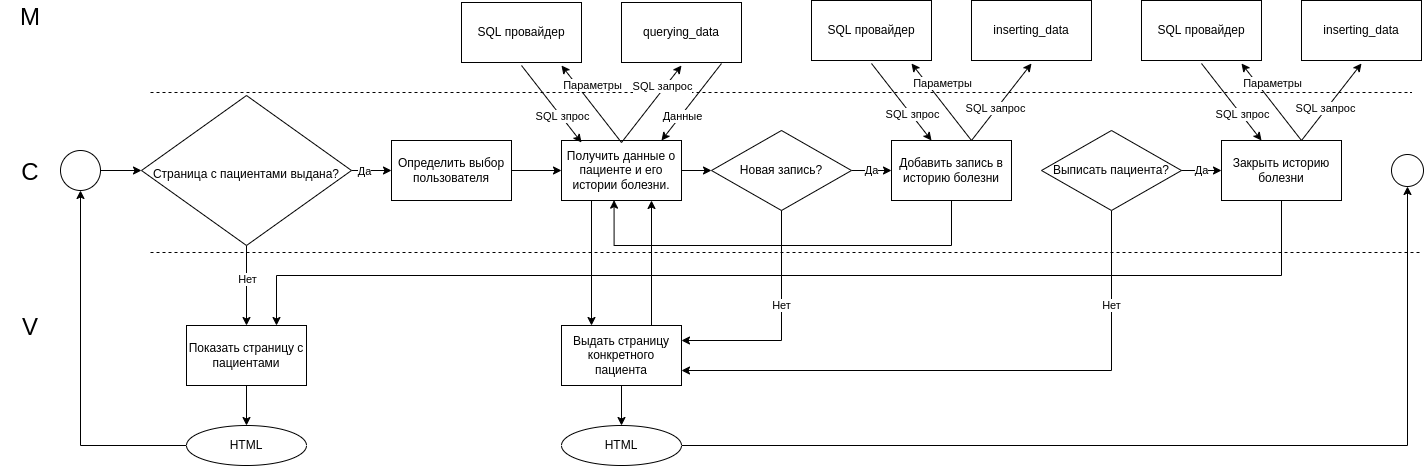
\includegraphics[width=1\textwidth]{pictures/treatment.png}
    	\label{fig:pic11} % Можно указывать ссылку на эту картинку в тексте, как \ref{fig:pic1}
    	\caption{BPMN диаграмма контроллера "Лечение пациента".}
    \end{figure}

    \subsection{Требования к шаблонам.}

    Данный сценраий реализации подрузамевает использование двух основных динамических таблиц, а именно: страница выбора паицента, страница лечения выбранного пациента.
    
    Страница выбора пациента должна содержать информацию о всех пациентах, для которых на данный момент открыта история болезни. Кроме того, данная страница должна предусматоривать разделение пациентов на две группы. Первая группа содержит пациентов, которые относятся к самому пользователю, а вторая, пациентов, относящихся к другим пользователям. Данные о каждом пользователе представлены в виде некоторого визуального объекта, содержащего кнопку "Провести осмотр". Нажав на эту кнопку пользователь передает параметры о выбраном пользователе в систему, которая в свою очередь открывает страницу лечения выбранного пациента.
    
    Страница лечения выбранного пациента должна содержать всю информацию о пациенте, его враче и истории болезни. Кроме того, на данной странице должен размещаться список записей в истории болезни.
    
    На странице лечения выбранного пациента должно быть две формы. Первая форма позволяет провести осмотр и внести новую запись в историю болезни. Эта форма должна содержать в себе текстовое поле ввода и кнопку для отправки данных в систему. Вторая форма необходима для выписки пациента. Она также содержит текстовое поле для внесения диагноза при выписке, а и кнопку для отправки данных в систему. При использовании первой формы, пользователь должен увидить отображение новой, внесенной им, записи на странице пациента. При использовании второй формы пользователя вернут на страницу выбора пациента. Однако, только что выписанного пациента в списке уже быть не должно, так как его история болезни закрыта.

    \newpage
    \subsection{Программная аритектура реализации сценария "Лечение пациента".}
    \begin{figure}[h]
    	\centering    % Центрируем
    	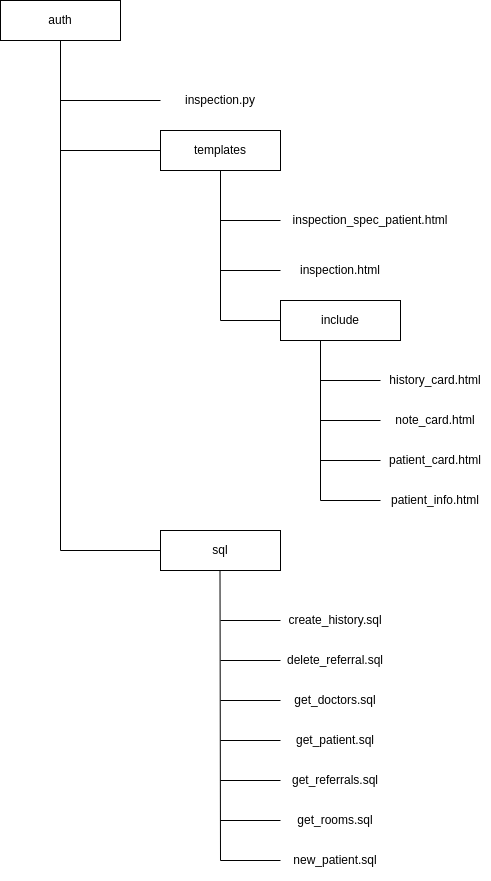
\includegraphics[height=0.7\textheight]{pictures/archTreatment.png}
    	\label{fig:pic12} % Можно указывать ссылку на эту картинку в тексте, как \ref{fig:pic1}
    	\caption{Программная аритектура реализации сценария "Лечение пациента".}
    \end{figure}

    \newpage
    \section{Логическая модель базы данных}
    \begin{figure}[ht!]
    	\centering    % Центрируем
    	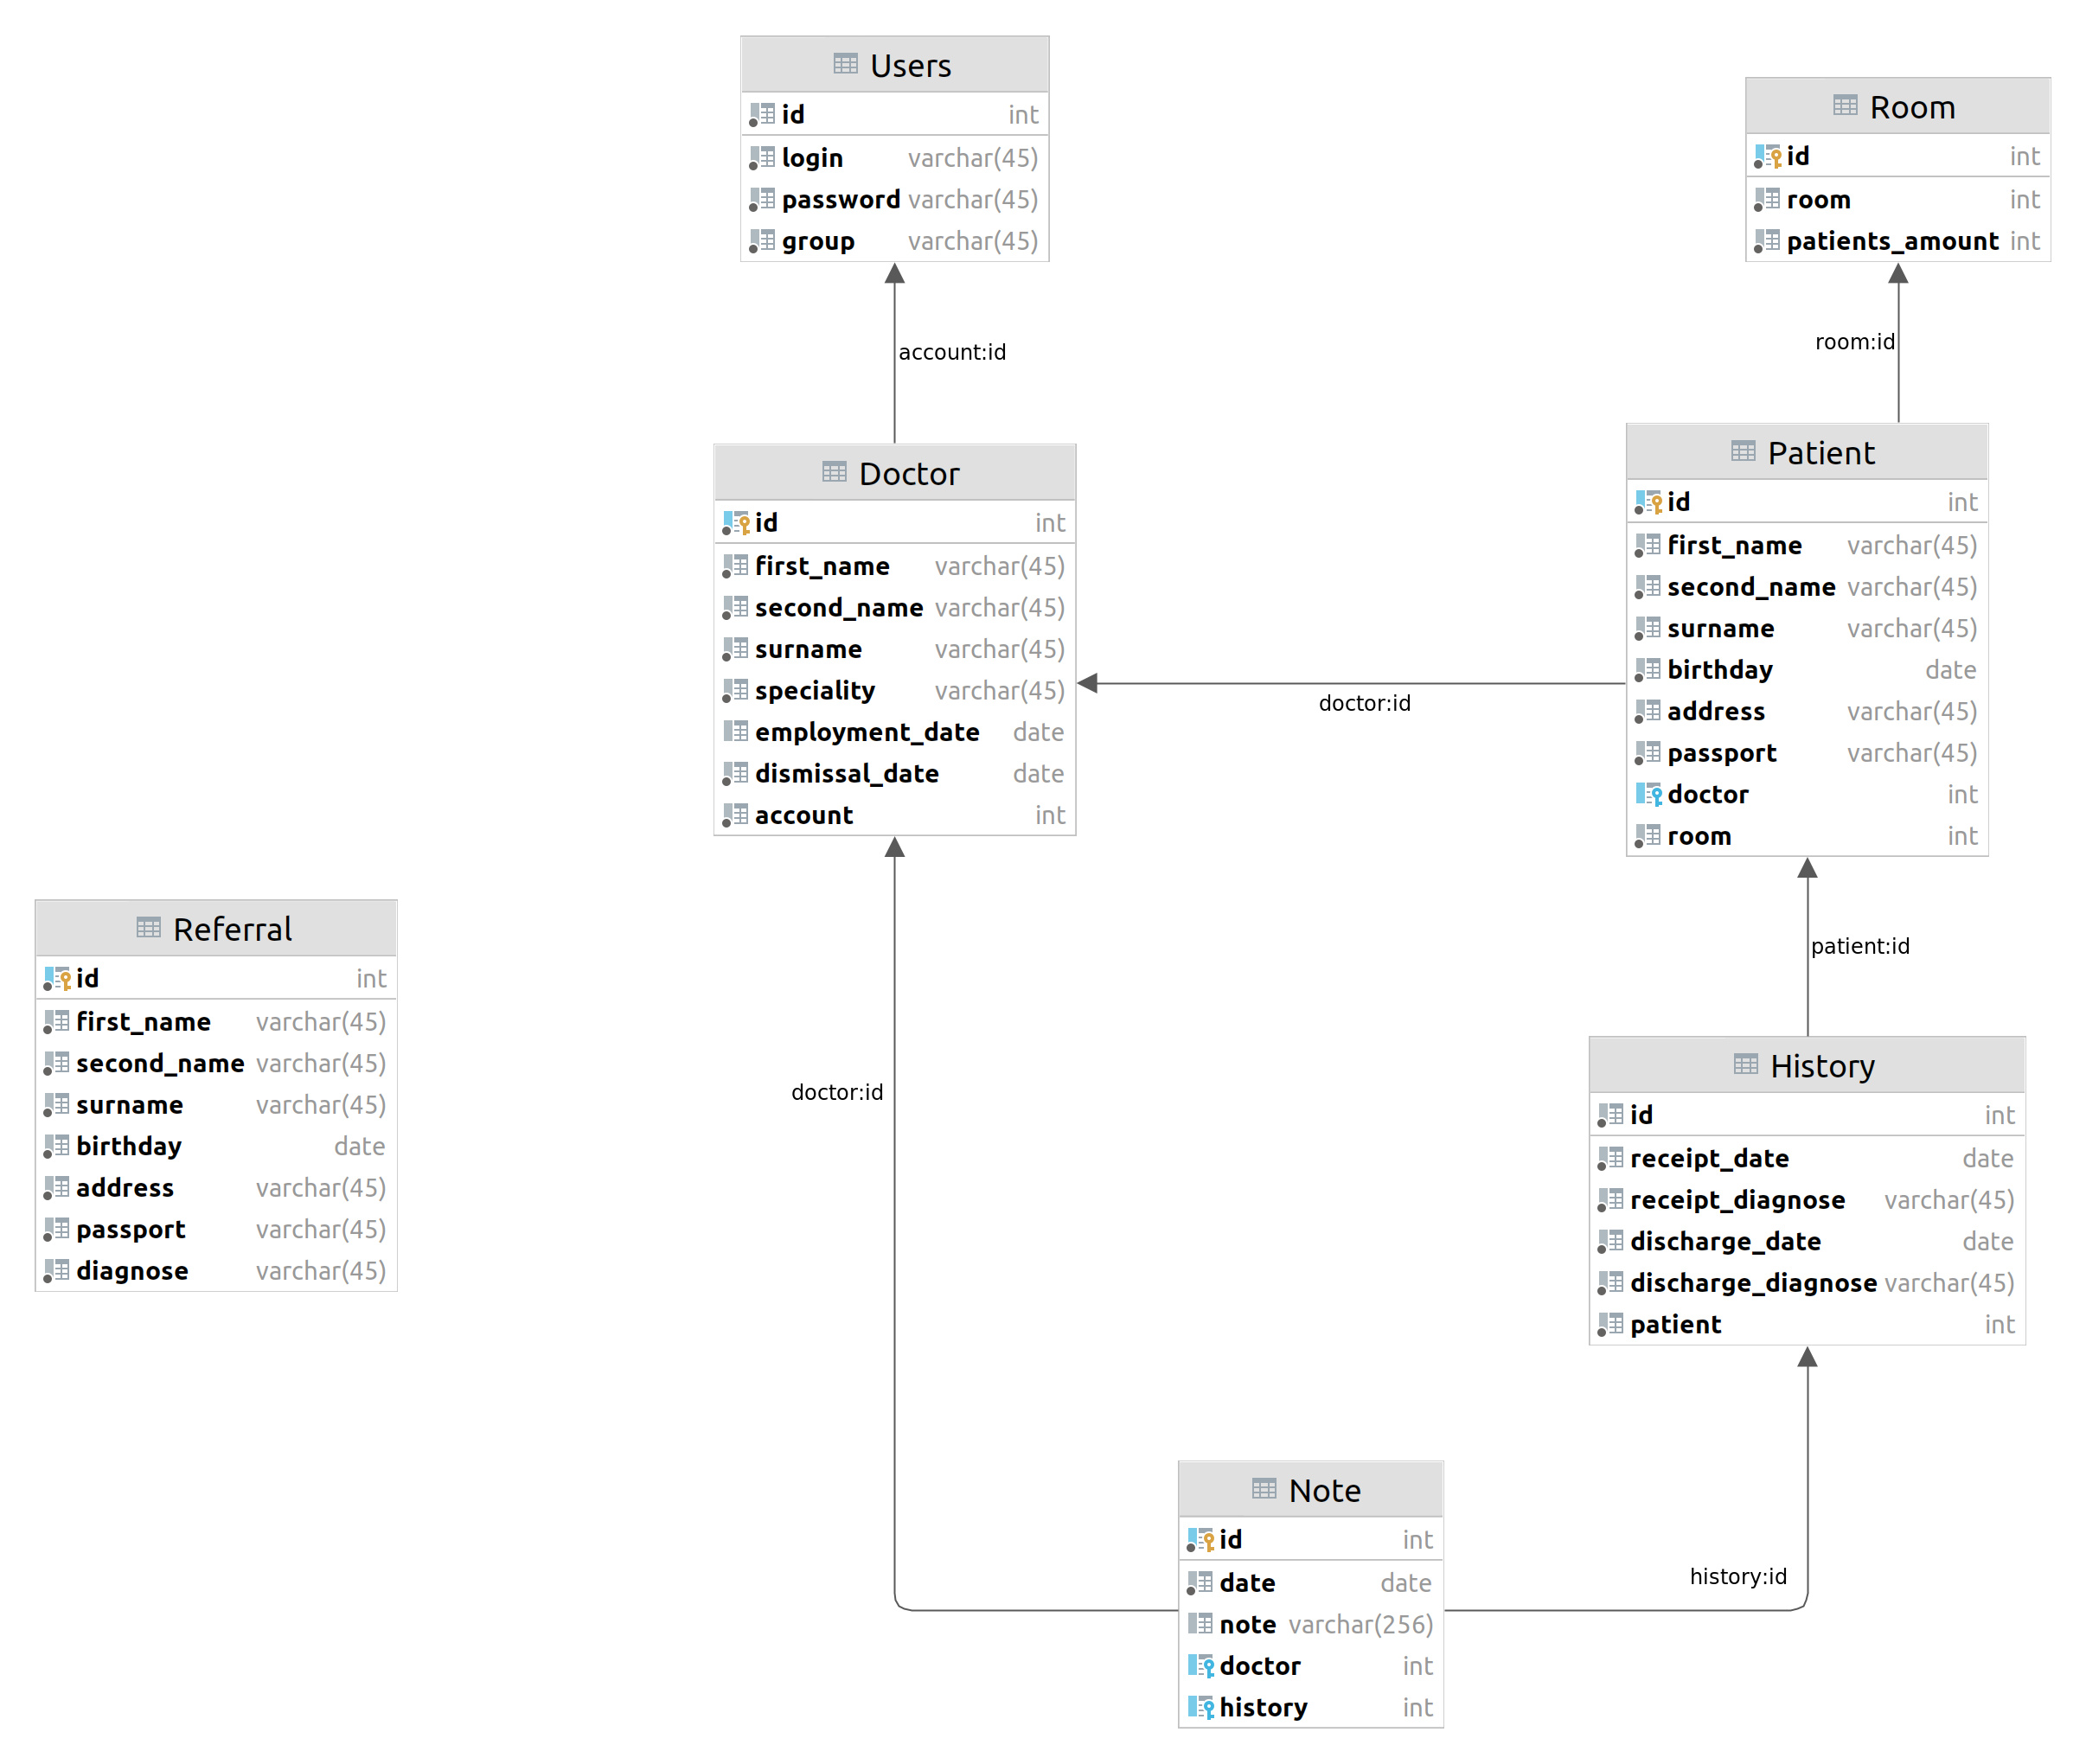
\includegraphics[width=1\textwidth]{pictures/logic_model.png}
    	\label{fig:pic13} % Можно указывать ссылку на эту картинку в тексте, как \ref{fig:pic1}
    	\caption{Логическая модель базы данных информационной системы "История болезни". Диаграмма.}
    \end{figure}
    
    \begin{table}[hb!]
    	\caption{Таблица Doctor}
    	\begin{center}
        	\begin{tabular}{ | l | l | l | l | l | l | l | l | }
        		\hline
        		\textbf{id} & f\_name & s\_name & surname & speciality & empl\_date & dis\_date & account \\ \hline 
        		pk & & & & & & & fk
        	\end{tabular}
        \end{center}
    \end{table}

    \begin{table}[hb!]
    	\caption{Таблица Patient}
    	\begin{center}
        	\begin{tabular}{ | l | l | l | l | l | l | l | l |l | }
        		\hline
        		\textbf{id} & f\_name & s\_name & surname & birthday & address & passport & doctor & room \\ \hline 
        		pk & & & & & & & fk & fk
        	\end{tabular}
        \end{center}
    \end{table}

    \newpage
    \begin{table}[ht!]
    	\caption{Таблица History}
    	\begin{center}
    		\begin{tabular}{ | l | l | l | l | l | l | }
   	 			\hline
    			\textbf{id} & receipt\_date & receipt\_diagnose & descharge\_date & descharge\_diagnose & patient \\ \hline 
    			pk & & & & & fk
    		\end{tabular}
    	\end{center}
    \end{table}

    \begin{table}[ht!]
    	\caption{Таблица Note}
    	\begin{center}
        	\begin{tabular}{ | l | l | l | l | l | }
        		\hline
        		\textbf{id} & date & note & doctor & history \\ \hline 
        		pk & & & & fk
        	\end{tabular}
       \end{center}
   \end{table}

    \begin{table}[ht!]
    	\caption{Таблица Users}
    	\begin{center}
    		\begin{tabular}{ | l | l | l | l | }
    			\hline
    			\textbf{id} & login & password & group \\ \hline 
    			pk & & &
    		\end{tabular}
    	\end{center}
    \end{table}

    \begin{table}[ht!]
    	\caption{Таблица Room}
    	\begin{center}
    		\begin{tabular}{ | l | l | l | }
    			\hline
    			\textbf{id} & room & patiens\_amount \\ \hline 
    			pk & &
    		\end{tabular}
    	\end{center}
    \end{table}
   
\end{document}